\documentclass[12pt]{article}

% Use reasonably small margins
\usepackage{fullpage}
\usepackage{mathtools}

% for various math utilities
\usepackage{amsmath}
\usepackage{amssymb}
\usepackage{commath}
\usepackage{cancel}
\usepackage{breqn}
\usepackage{eurosym}

% provides non-italicized Greek letters in text
\usepackage[euler]{textgreek}

% provides the \includegraphics command
\usepackage{graphicx}
\usepackage{subfig}

% allows figure environments to be placed in exact locations
\usepackage{float}

% Bold caption labels, and give captions increased margins
\usepackage[labelfont=bf, margin=1cm]{caption}

% allows for configurable source code listings
\usepackage{listings}
\usepackage{color}
\definecolor{dkgreen}{rgb}{0,0.6,0}
\definecolor{gray}{rgb}{0.5,0.5,0.5}
\definecolor{red}{rgb}{0.8,0,0}
\lstset{frame=tb,
  language=C,
  aboveskip=3mm,
  belowskip=3mm,
  showstringspaces=false,
  columns=flexible,
  basicstyle={\small\ttfamily},
  numbers=left,                    % where to put the line-numbers; possible values are (none, left, right)
  numbersep=5pt,                   % how far the line-numbers are from the code
  numberstyle=\tiny\color{gray},   % the style that is used for the line-numbers
  stepnumber=1,                    % the step between two line-numbers. If it's 1, each line will be numbered
  keywordstyle=\color{blue},
  commentstyle=\color{dkgreen},
  stringstyle=\color{red},
  breaklines=true,
  breakatwhitespace=true,
  breakindent=50pt,
  tabsize=4
}

% allows hyperlinks
\usepackage{hyperref}


\begin{document}

\begin{titlepage}
\begin{center}

\textsc{\LARGE Internet of Things} \\[0.5cm]

\emph{\LARGE Universit{\"a}t Bremen } \\[5cm]

{\huge \bfseries Final Project Report: \\ SubSpy} \\[3cm]

{\LARGE Marcio Jose de Menezes Junior }\\[0.5cm]

{\LARGE Student ID: 3109694}


\vfill

{\LARGE Bremen, July 27th, 2017}

\end{center}
\end{titlepage}


\newpage

\tableofcontents

\vfill
\newpage

%--------------------------------------------------
% INTRODUCTION TO SUBSPY
%--------------------------------------------------


\section{Introduction}

%TODO: Write initial part of introduction?
SubSpy is a wireless adapter card designed to promiscuously listen on a sensor network providing means to extract data packets from the target network. The data card streams the incoming data packets through a USB communications device class (CDC) interface which is compatible with Linux, Windows, Mac and Android devices.

The wireless communication interface is build around HOPERF's radio transceiver RFM69CW while the host MCU is based on Texas Instruments MSP430F5529 which has a built-in USB interface as well as all other relevant peripherals.

An user interface designed with QT is available for Windows and Linux which is capable of logging the packets into text files as well as plotting the sensor's readings.

%--------------------------------------------------
% SYSTEM DESIGN
%--------------------------------------------------

\section{System Architecture}
\label{systemArch}

The system architecture design process consisted of analysing the high level requirements presented on the IoT challenge, and translating them into a high level hardware abstraction in order to establish the main components to be further developed on the hardware design phase.

The solution architecture is straightforward consisting of two main components, the RFM69CW radio transceiver and the MSP430F5529 microcontroller. The RFM69CW is a RF transceiver module capable of operation on the 315, 433, 868 and 915MHz license-free ISM frequency bands, this project uses the variant configured to operate on the 433MHz band. 

The MSP430F5529 is a 16-bit low power microcontroller which features an integrated USB communications interface and has been selected due to its superior performance and low power consumption if compared to AVR microcontrollers. The selected microcontroller also features several integrated hardware peripherals such as UART, SPI, DMA, RTC, integrated LDO among others, its integrated USB interface eliminates the need for an external USB bridge, which can be not only costly but also power hungry, as it is the case with most development kits.

\newpage
Figure~\ref{fig:subSpyArchitecture} depicts the high level architecture of the proposed solution.

\begin{figure}[H]
    \centering
    \includegraphics[width=1.0\textwidth]{subSpyArchitecture.png}
    \caption{SubSpy High Level System Diagram.}
    \label{fig:subSpyArchitecture}
\end{figure}

%\newpage
Furthermore, the designed solution contains 3 indication LEDs, the first one represents messages transmitted to the host (hand held device), the second one the messages received from the host and the last one is a RGB LED which is meant to be used to indicate the wireless captured packets as well as generic system status indication.
The solution contains three tactile switches for user interaction, being the BSL switch responsible to enable the USB bootstrap-loader for firmware update on the field, RST switch to generate hardware resets and USR switch which is available for user custom functions. Additionally there is an external 32M-bit  flash memory which enables standalone operation meaning that a hand held device is not necessary to collect the data, it can be retrieved later at user convenience through the USB interface.
The external flash memory as well as the RFM69CW are accessed through SPI serial interface, which is fully handled by hardware SPI on the MSP430F5529 microcontroller.

\newpage
\section{Hardware Design}
\label{hardwareDesign}
To produce a solution which was cost effective, energy friendly, and still offered high throughput, it has been decided that a development kit would be used only for the purpose of creating a proof of concept (prototype), the final solution would have a custom made PCB with optimized size and shape.

The PCB design has been created on EAGLE and the schematic is split in 2 parts, Figure~\ref{fig:subspySchematics} contains the main part of the PCB design which holds the MCU as well as the USB circuitry. Additionally, it has two quartz crystal references, one low frequency 32768Hz used by the real time clock system (RTC) and another high frequency (4MHz) which is used to generate a reference for the USB 48MHz PLL and for the MCLK and SMCLK which drive the MSP430 core and peripherals respectively. Additionally the design also includes a SPY-BY-WIRE interface (2-wire debug protocol) which enables real time debugging using Texas Instruments Code Composer Studio. Additional GPIOs are also available should the user need to connect additional sensors or control actuators.

\begin{figure}[H]
    \centering
    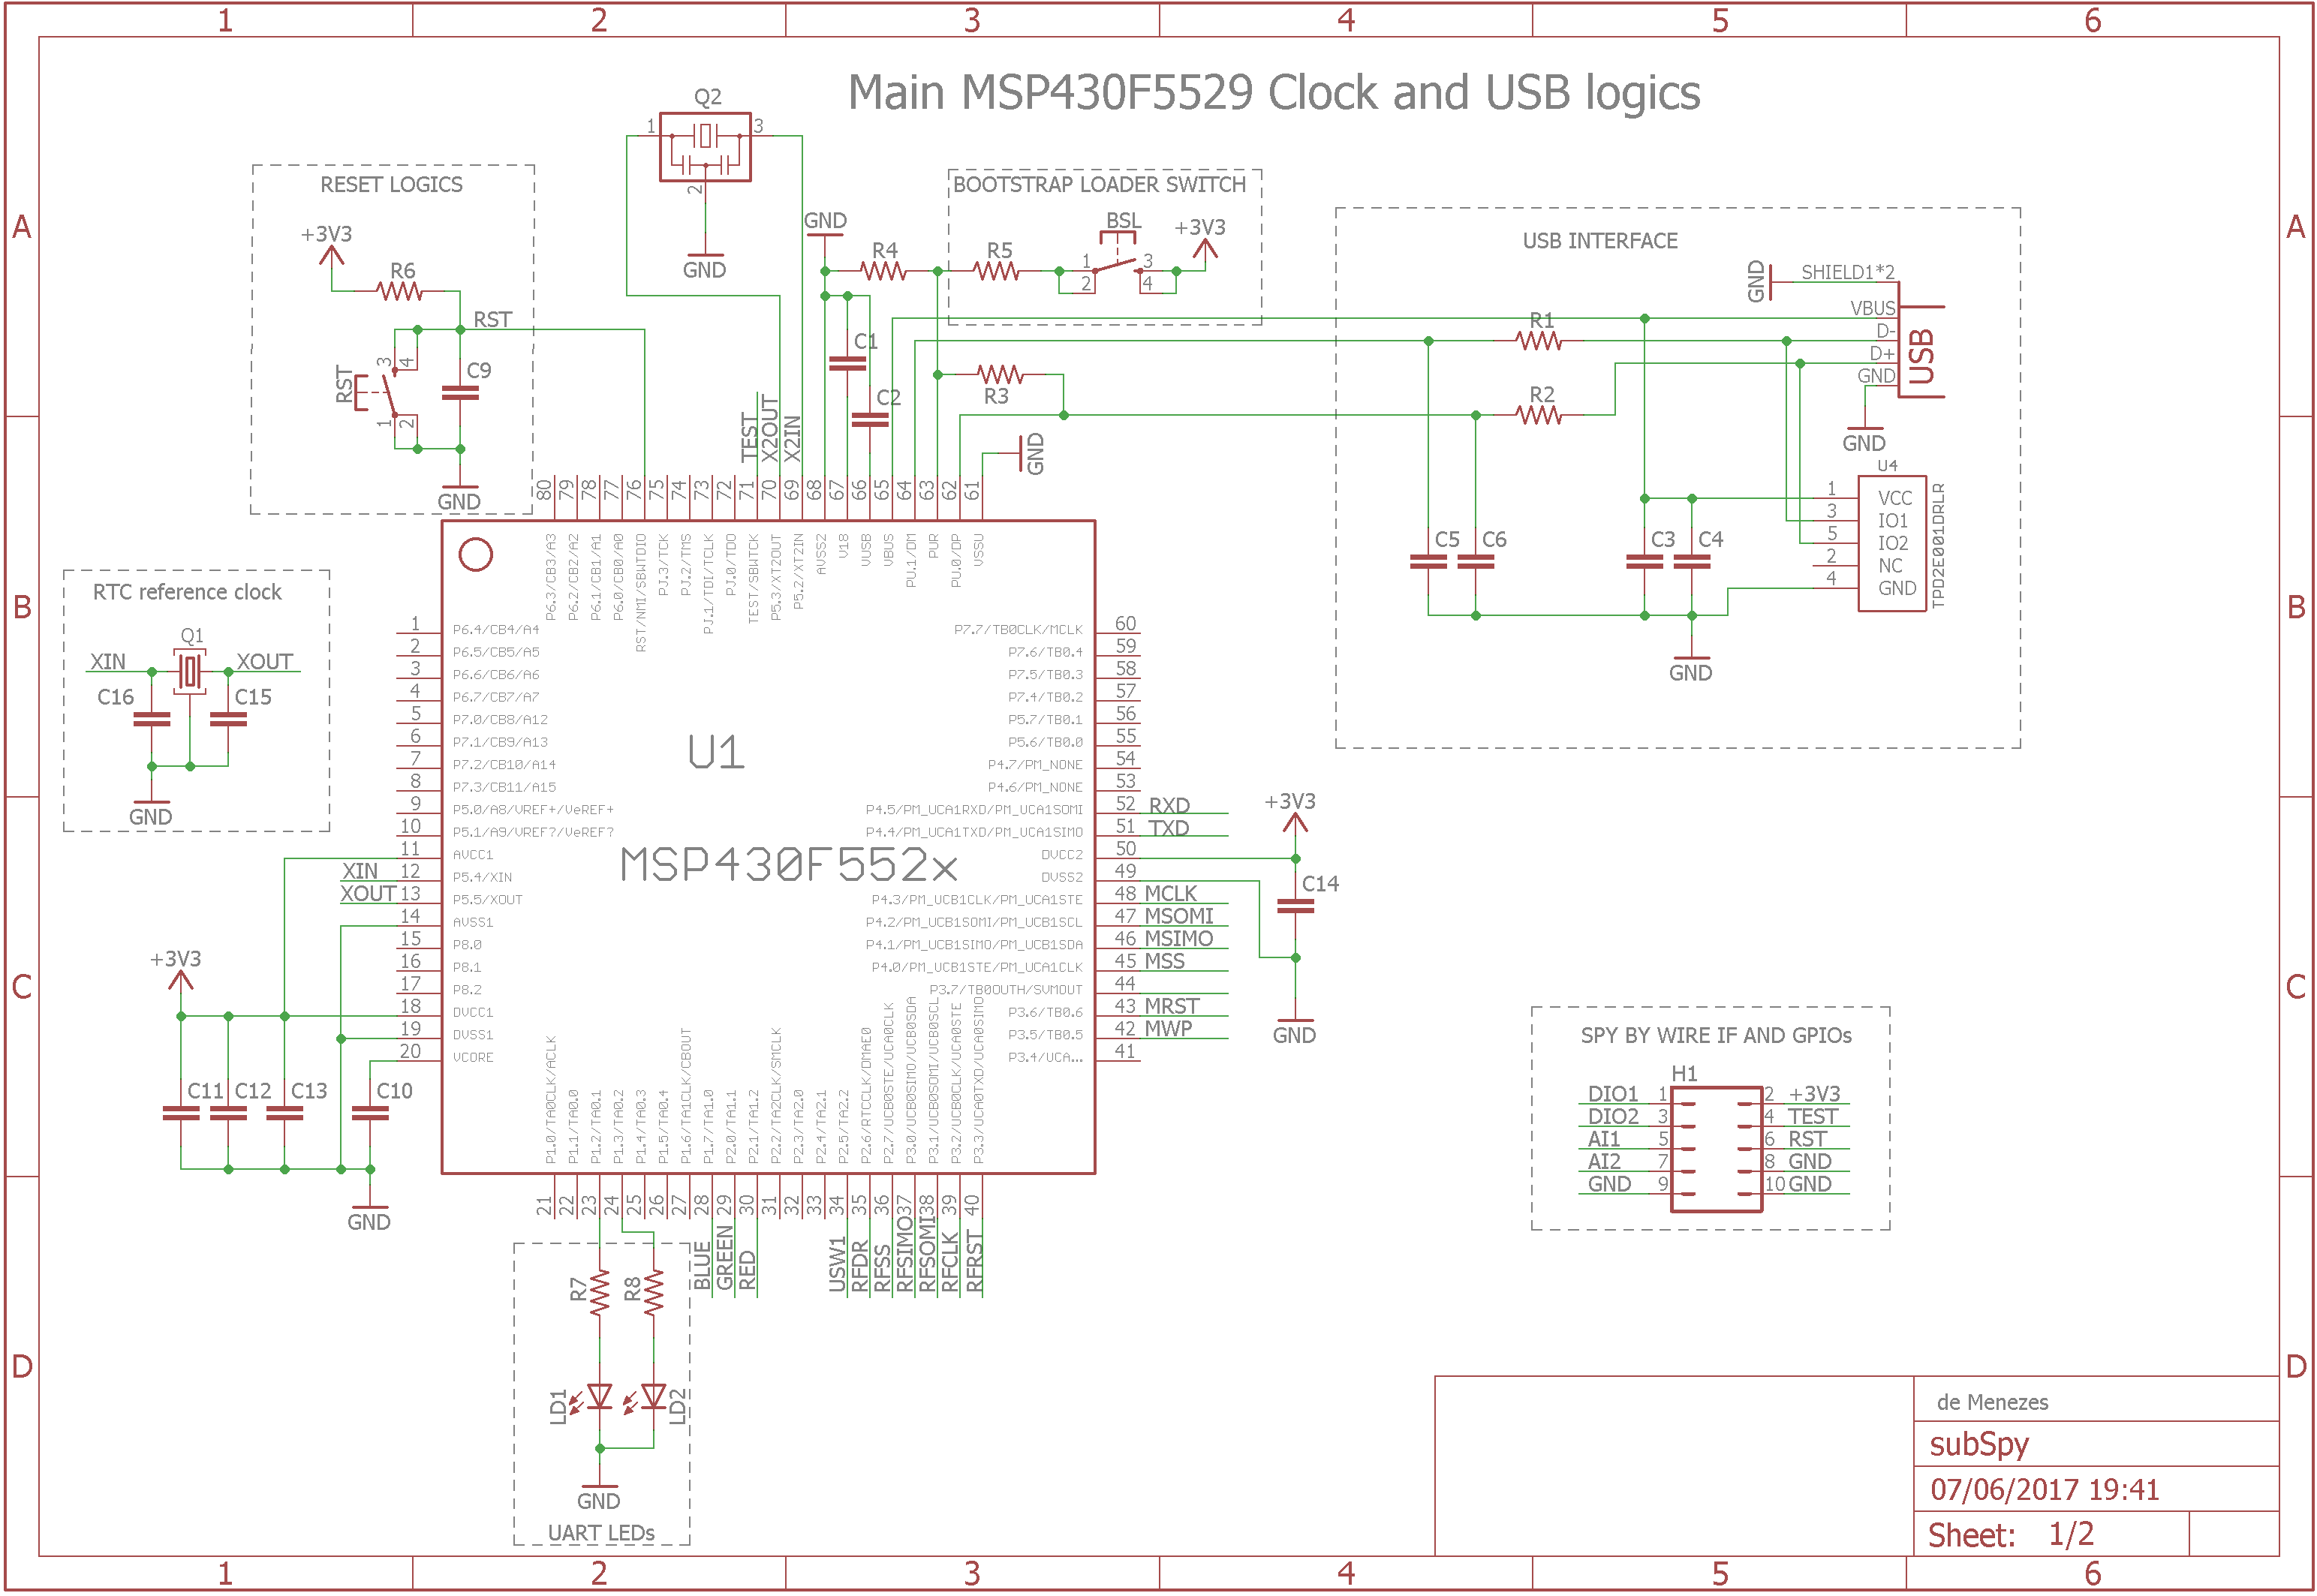
\includegraphics[width=1.0\textwidth]{subspySchematics.png}
    \caption{MCU and USB logics schematic.}
    \label{fig:subspySchematics}
\end{figure}

\newpage
The second schematic partition on Figure~\ref{fig:subspySchematics2} contains the DC/DC power supply, RFM69CW radio interface, external flash, RGB indication LED as well as the user switch.

\begin{figure}[H]
    \centering
    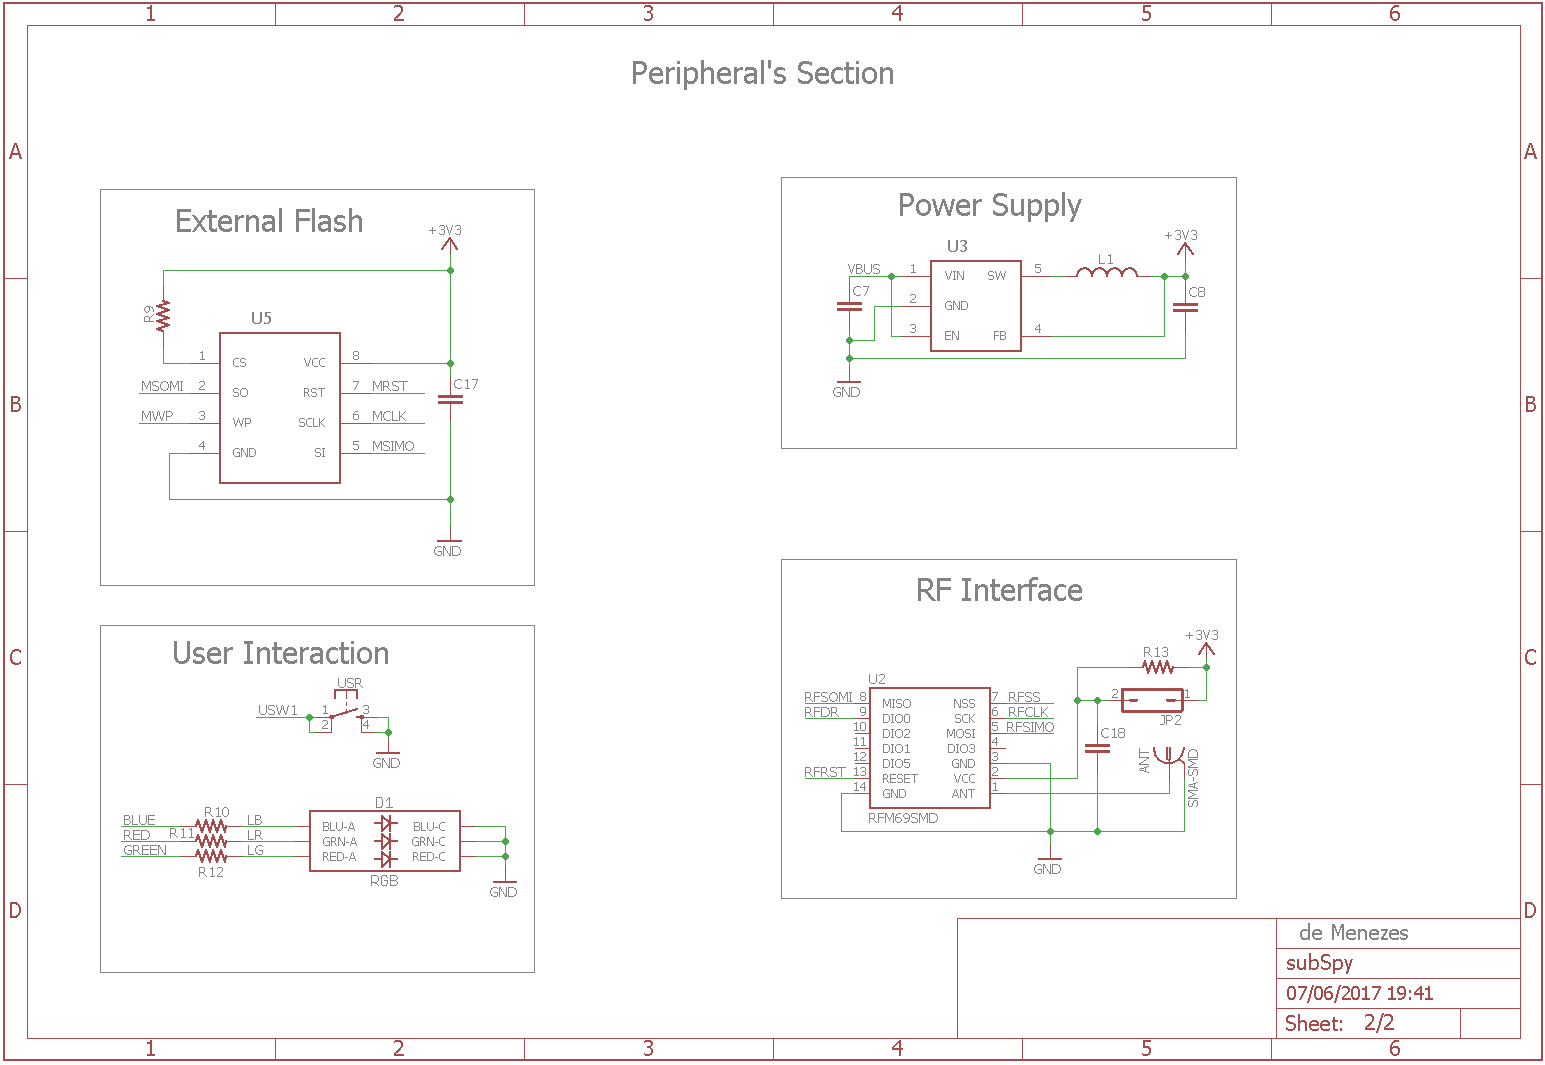
\includegraphics[width=1.0\textwidth]{subspySchematics2.png}
    \caption{Peripheral schematic.}
    \label{fig:subspySchematics2}
\end{figure}

\newpage
Despite the fact that MSP430F5529 already has an integrated LDO regulator (which means that 3.3V could be directly derived from the 5V USB bus without the need of an external regulator), it has been decided to design an external switching power supply.
To uncover the rationale for this decision, it is necessary to understand that the integrated LDO is a linear regulator, which has good efficiency under light load operation (e.g. MCU in sleeping mode) and compared to other linear topologies is a reasonable choice in many cases, specially because there is no need of external components, a fact that not only reduces BOM cost but also reduces system footprint. 

In general, the efficiency of DC/DC converters are close to LDOs under light load conditions but as the current consumption grows, the DC/DC becomes much more efficient than the LDO. As the SubSpy project features a radio interface which alone in listening mode will draw around 16mA from the 3V3 power supply, it becomes inevitable to consider a more efficient power supply given the power consumption constraints. It has been identified a possibility to save up to 40\% (depending on the operating point) on power losses if an external DC/DC buck converter was implemented. Figure~\ref{fig:DCDC_VS_LDO} compares the overall current consumption between LDO and DC/DC converter in a similar device for different operating frequencies. 

\begin{figure}[H]
    \centering
    \includegraphics[width=0.9\textwidth]{DCDC_VS_LDO.png}
    \caption{DC/DC Vs LDO.}
    \label{fig:DCDC_VS_LDO}
\end{figure}

The final PCB design is illustrated on figure~\ref{fig:subspyBoard}, as can be observed the solution achieved a reasonably good size and shape and Figure~\ref{fig:spyPreview} depicts a 3D rendering preview of the final design. The bill-of-materials (BOM) cost settled around \euro 25 to produce small quantities (less than 10 units), including shipping costs, taxes and the PCB, but excluding the PCB assemble costs, which is a good value considering the alternative of using development kits which are not tailored for the application, deliver worst performance with higher current consumption.

\begin{figure}[H]
    \centering
    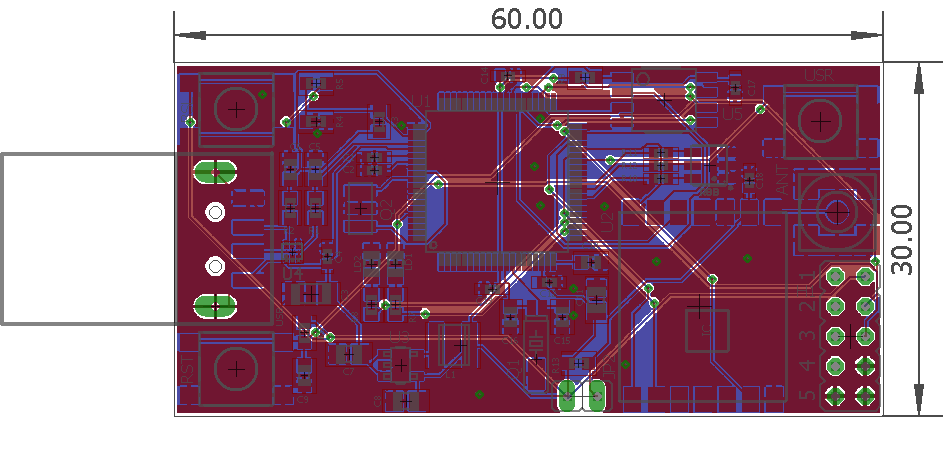
\includegraphics[width=0.75\textwidth]{subspyBoard.png}
    \caption{Designed PCB.}
    \label{fig:subspyBoard}
\end{figure}

\begin{figure}[H]
    \centering
    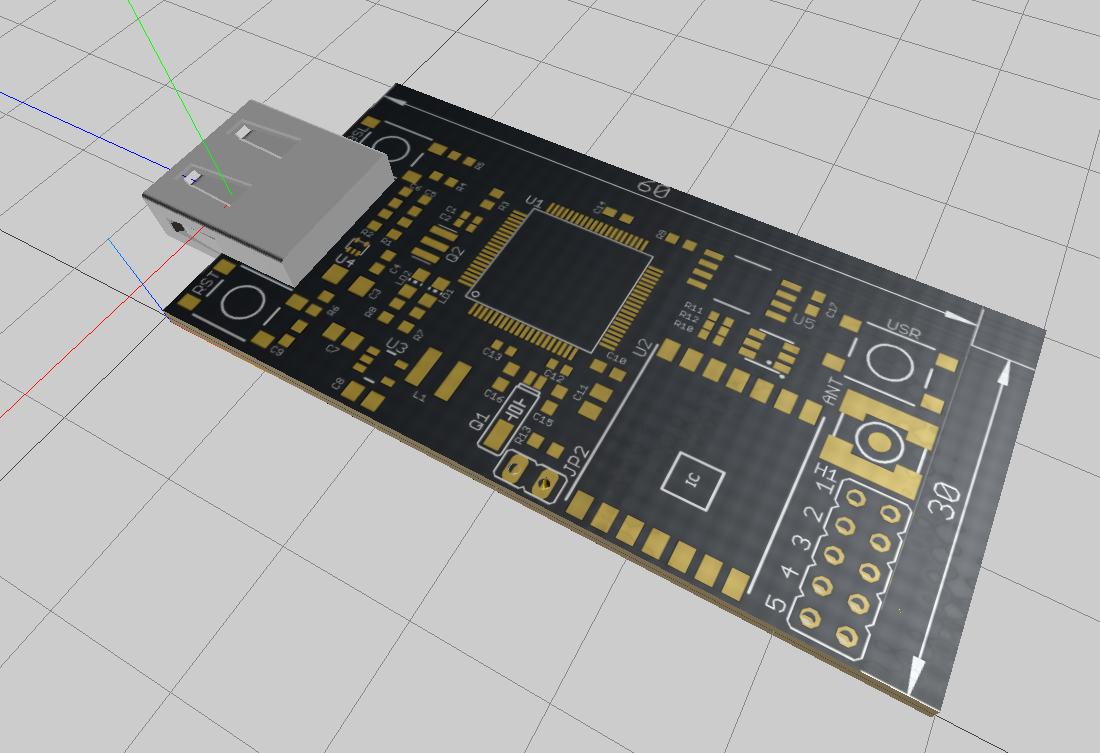
\includegraphics[width=0.75\textwidth]{spyPreview.png}
    \caption{3D rendering preview.}
    \label{fig:spyPreview}
\end{figure}

\newpage
\section{Proof of Concept}
\label{proofOfConcept}
As time was a great constraint for the project, it has been decided that the PCB would only be ordered after a fully functional proof of concept had been developed and evaluated. For this purpose, the development kit MSP-EXP430F5529LP from Texas Instruments has been selected. This kit is part of a development environment called Lauchpad (slightly similar to what Arduino represents for Atmel) which releases several development kits featuring microcontrollers from TI.

The development board has a header interface which developers can use to access the GPIOs of the target MCU. This interface has standardized pinout and peripheral connections allowing to connect several community BoosterPacks, which are satellite boards with extended functionality featuring different ICs providing a fast track development environment for seamless applications.

As there is no RFM69CW BoosterPack available, one has been developed using a fast prototyping board in order to create a fully functional prototype for the final project. Figure~\ref{fig:prototype} illustrate the final prototype used to validate the proposed hardware solution.

\begin{figure}[H]
    \centering
    \includegraphics[width=1.0\textwidth]{prototype.png}
    \caption{MSP-EXP430F5529LP with RFM69CW home made BoosterPack.}
    \label{fig:prototype}
\end{figure}


\newpage
\section{Firmware Implementation}
\label{firmwareImplementation}
The main challenge about leaving the usual Arduino solution to migrate to the MSP430 platform regards the RFM69CW radio protocol library which is available for Arduino but not for MSP430 and therefore required a full port into C programming language. This sort of code porting is often not a problem, however, due to time limitations it was a great challenge to be successfully accomplished and to have a the fully operational prototype ready on schedule.

Regarding the USB implementation, TI provides a complete API for the USB peripheral, it has been decided to implement the wireless adapter as a communications device class (CDC) since it is simple enough and doesn't require any specific driver to be installed on either Windows (from Windows 7 onwards) or Linux (also applies for Android and Mac).

The following sub-sections will introduce additional functionality implemented on SubSpy firmware as well as introduce the overall device operation.


\subsection{Device Operation}
Besides the main routine, the wireless adapter has another two important routines, regarding the promiscuous listening task, the gatewayPassiveListen and the gatewayActiveListen.

The main routine basically initializes the low level registers for system's peripherals such as RTC, clock domain, references, system timers, core voltage, GPIOs and USB interface. It also performs a clean initialization (reset) of the RFM69CW radio transceiver.

After the system is properly initialized the MCU goes into sleep mode and waits until the host device has enabled the wireless adapter. There are two possibilities for the listening operation. The first is implemented by gatewayPassiveListen and it is designed to put the radio interface in sleep mode accordingly to a user configurable duty cycle, enabling further energy savings. This approach may be useful for some use cases where the network load is high at some intervals and low or non-existent in others. It has the penalty that a few packets may be lost until the radio has detected network activity, higher duty cycles will reduce the probability of packet losses. The duty cycle is configured by the user through the available user interface.

The second listening operation is actually a sub-routine of gatewayPassiveListen and it is called gatewayActiveListen. This is the operation mode engaged when network activity is detected and it is the same regardless the duty cycle selection, in this mode the radio transceiver duty cycle is 100\%. Thus, the radio duty cycle selection only affects the program behaviour if there is no network activity detected.
  
\begin{figure}[H]
    \centering
    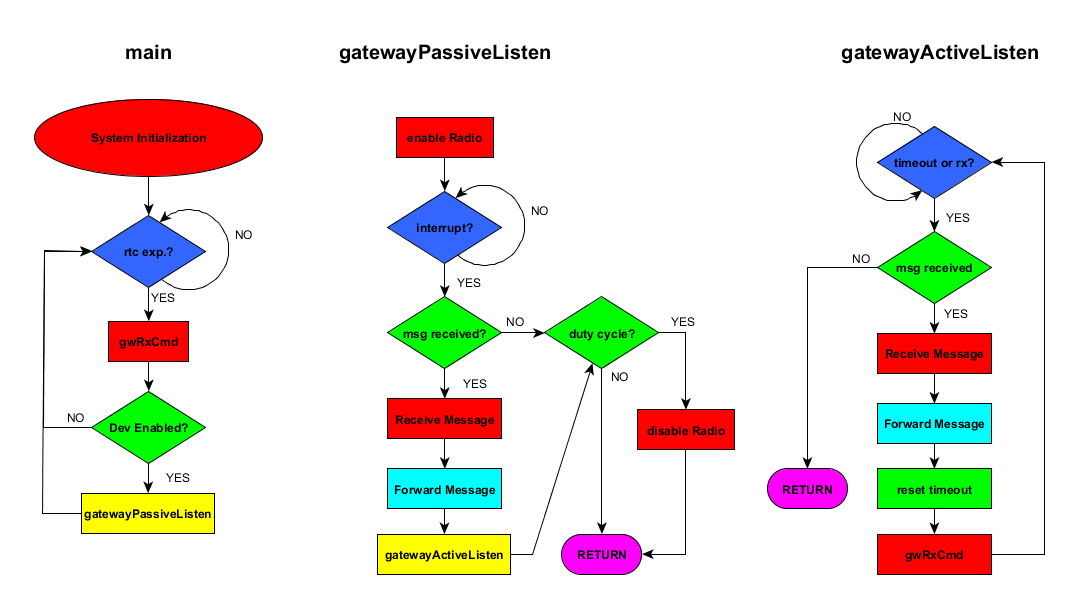
\includegraphics[width=1.0\textwidth]{subspyProgramFlow.png}
    \caption{SubSpy program flowchart.}
    \label{fig:subspyProgramFlow}
\end{figure}

Figure~\ref{fig:subspyProgramFlow} depicts the program flow of the implemented routines and has merely the intention to give a high level idea of the implementation. Unfortunately time constraints have made impossible to write software requirements for the implementation and therefore more information is available only on source code and comments.

\subsection{Field Firmware Upgrade}
The SubSpy has been designed to ensure easy firmware upgrade on the field. This procedure is accomplished by the BSL switch, which should be pressed simultaneously while connecting the wireless adapter to a USB host. Pressing the switch at power up time will activate the ROM USB bootstrap-loader which will enumerate the device as a mass storage unit and it will mount on the system as if it were a flash memory stick. In this way, to reprogram the firmware the user just have to drag and drop the .hex file (firmware) on the mass storage device and it will be promptly flashed, without the need of a Code Composer Studio installation and a flash loader hardware.

\subsection{Low Power Mode and Clock Design}
The MSP430 has several configurable low power modes available, however, most of them are not available if the USB peripheral is active since some circuitry cannot be shut down otherwise the host device would loose the USB enumeration of the wireless adapter.
For this reason, the only low power mode used throughout the application is the LPM0 which basically shuts down the MSP430 core, keeping all clocks and peripherals in normal operation. But this is not a disadvantage as it may look like, while the MCU wastes a couple micro-Amps by not gating the clocks in sleep mode, the integrated USB peripheral saves a few milli-Amps compared to the external USB bridge alternative.

Besides the simple activation of low power modes, battery sensitive applications need to be perfectly trimmed regarding power consumption. The current draw has to be carefully evaluated through representative benchmarks considering all use cases to determine the optimal operational point where we can achieve the best battery yield keeping the required system performance. This project has approached different energy saving techniques which are described in sequence.

\subsubsection{RAM Program Code Execution}
By default the program code is always placed on the MCU integrated flash memory by the linker, flash memory reading operation however consumes as much as 300\% more than RAM memory reading. Considering this, if commonly accessed routines are moved from flash to RAM in run time, it is possible to cut current consumption significantly. Naturally this approach is tied to additional overhead but in general it is possible to find a good balance and save a considerable amount of energy. The Code Composer Studio's compiler already performs some optimization (if configured) to run some common code from RAM, like operations implemented by the run time library such as software floating point operations and others.

\subsubsection{System Clock Design}
The MSP430F5529 can operate at up to 25MHz if using the integrated Digitally Controlled Oscillator (DCO) as reference for the FLL circuitry or 24MHz with an external 4 or 8MHz reference. Naturally, the MSP430 is a CMOS based device and therefore as the operating frequency increases so does the current due to the charging and discharging of load capacitances intrinsic on MOSFET's gate and the instant short circuits during logics transition. In the other hand, increasing the core frequency will also increase system throughput and therefore the system will process its tasks faster and spend more time on sleep mode. In order to find the optimal operating point, several benchmarks have been performed in order to gather information about different clock setups.

Figure~\ref{fig:clockCurrent} shows the MCU current consumption according to operating frequency using the DCO as reference. The external reference has also been evaluated and the DCO has presented better results regarding energy efficiency although the difference is quite small. It can be observed that the current consumption profile is almost linear, with a slight increase after 20MHz.

\begin{figure}[H]
    \centering
    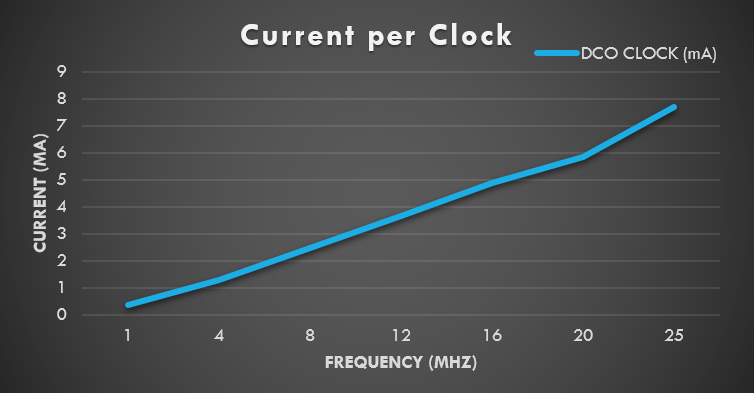
\includegraphics[width=0.7\textwidth]{clockCurrent.png}
    \caption{Clock current consumption.}
    \label{fig:clockCurrent}
\end{figure}

Considering the program execution time linearly proportional to the system clock (what is a reasonable approximation for THIS application), it makes sense to target the system clock to the frequency which will yield the smallest cost (uA/MHz), figure~\ref{fig:clockCost} illustrates the clock cost for different configurations. We can observe that the clock cost decreases up to 20MHz and after that it starts to increase again. The reason for this behaviour is related to the fact that the MCU core voltage has to be increased from 2V2 to 2V4 in order to be able to operate above 20MHz and in consequence the higher voltage also increases the core losses upon switching.

\begin{figure}[H]
    \centering
    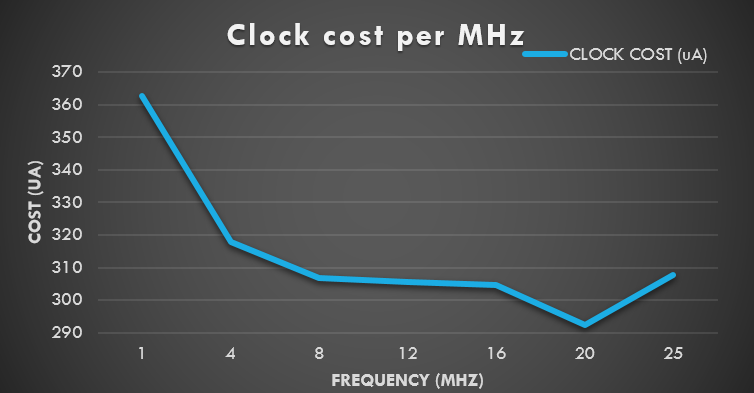
\includegraphics[width=0.8\textwidth]{clockCost.png}
    \caption{Clock cost uA/MHz.}
    \label{fig:clockCost}
\end{figure}

The tempting choice would be to fix the system frequency at 20MHz, however there are two other considerations to be made. The first one is related to system throughput, under heavy network loads, the wireless card could likely start missing packets, even thought it had capacity to run faster. Lab experiments revealed that the prototype can handle 647 packets/second operating at 25MHz and around 525 packets/second if operating at 20MHz. The second problem is related to the fact that the system clock cannot be switched off in sleep mode due to USB enumeration, in this case, it is desired that the clock speed should be as low as possible, just to maintain the USB peripheral in normal operation.

In the light of these constraints, it becomes evident that the optimal solution would be a dynamic clock reconfiguration routine which would change the clock setup on the fly, permitting the clock to be scaled down prior to entering sleep mode and scaled up accordingly to network activity. This routine has been implemented but is currently unstable since the dynamic clock reconfiguration requires adjustment of the core voltage on the fly, as well as settling routines to allow the FLL to stabilize after a reconfiguration in order to not generate erroneous non-maskable interrupts due to misinterpreted oscillator faults.

\subsubsection{Radio Data Reading Optimization}
Regarding the RFM69CW there is small room to improve operation efficiency besides the adjustable listening duty cycle, since the transceiver must remain in RX mode if gatewayActiveListen is engaged. There is however an exception hidden on the way the digital circuitry architecture has been devised on RFM69CW, whenever the internal registers are being read through the SPI interface, the transceiver is not able to receive a new packet from the analog circuitry. So if a packet is to be received while the data is being read out from the transceiver, this packet is going to be lost. Since the packet will be lost anyway, it is possible switch the radio from RX mode into sleep mode until the packet has been received and immediately after put it back on RX mode. 

The RFM69CW reading latency is inferior to 1.5ms, so during this time it is possible to cut down the overall system current by 16mA. However the overall savings will depend on the network activity, low traffic will force the radio to stay more time ON while high traffic will permit the radio to be in sleep mode more often (whenever a packet is being transferred to the MCU). By following this approach, it was possible to cut the average current draw by 15\% at a receiving rate of around 125 packets/second (one sensor node transmitting in burst mode).

\subsubsection{Other Approaches}
Finally, other small optimizations have been performed being two of them worth to mention. The first one is the usage of the direct memory access (DMA) peripheral, which allows to directly transfer the MCU's SPI registers content to the USB RAM with minimal CPU intervention, that means that while data is being received from the radio and placed on the USB memory, the CPU is in sleep mode saving up power. The second one is more trivial since it's basically the choice of what API method to use from the USB stack to transmit the data to the host, there is more than one method available and a good choice for this application is the background transmission in which the USB peripheral handles the data transmission leaving the MCU free to do as it pleases, be it sleep or receive a new packet.

\newpage
\section{The User Interface}
\label{userInterface}
Per requirement, the graphical user interface (GUI) is expected to log the data captured by the wireless adapter and eventually to plot the sensor readings. The user interface can also write commands on the spy itself, for instance to configure the radio duty cycle or to enable/disable indication LEDs. Although it is not implemented, it would be also possible to transmit data from the spy into the network under surveillance for purposes such as Over-The-Air firmware update (OTA), transmission rate/power reconfiguration among others.

The user interface has been implemented using QT, it has been decided to be so since it is a cross platform framework which enables the direct build release for Windows and Linux (also MAC, but not used in this project) platform without any need for additional programming. QT also has excellent documentation, a vast collection of libraries, it has been around for over 20 years and is also available under open source GPL license.

After the selection of the framework to develop the UI, the high level requirements for the final application have been evaluated and then translated into use cases and a prototype has been built. From the initial prototype an iterative process took place in order to further refine the solution since feedback from the possible stakeholders was not available. The final UI is presented in figure~\ref{fig:swWindows}.

\begin{figure}[H]
    \centering
    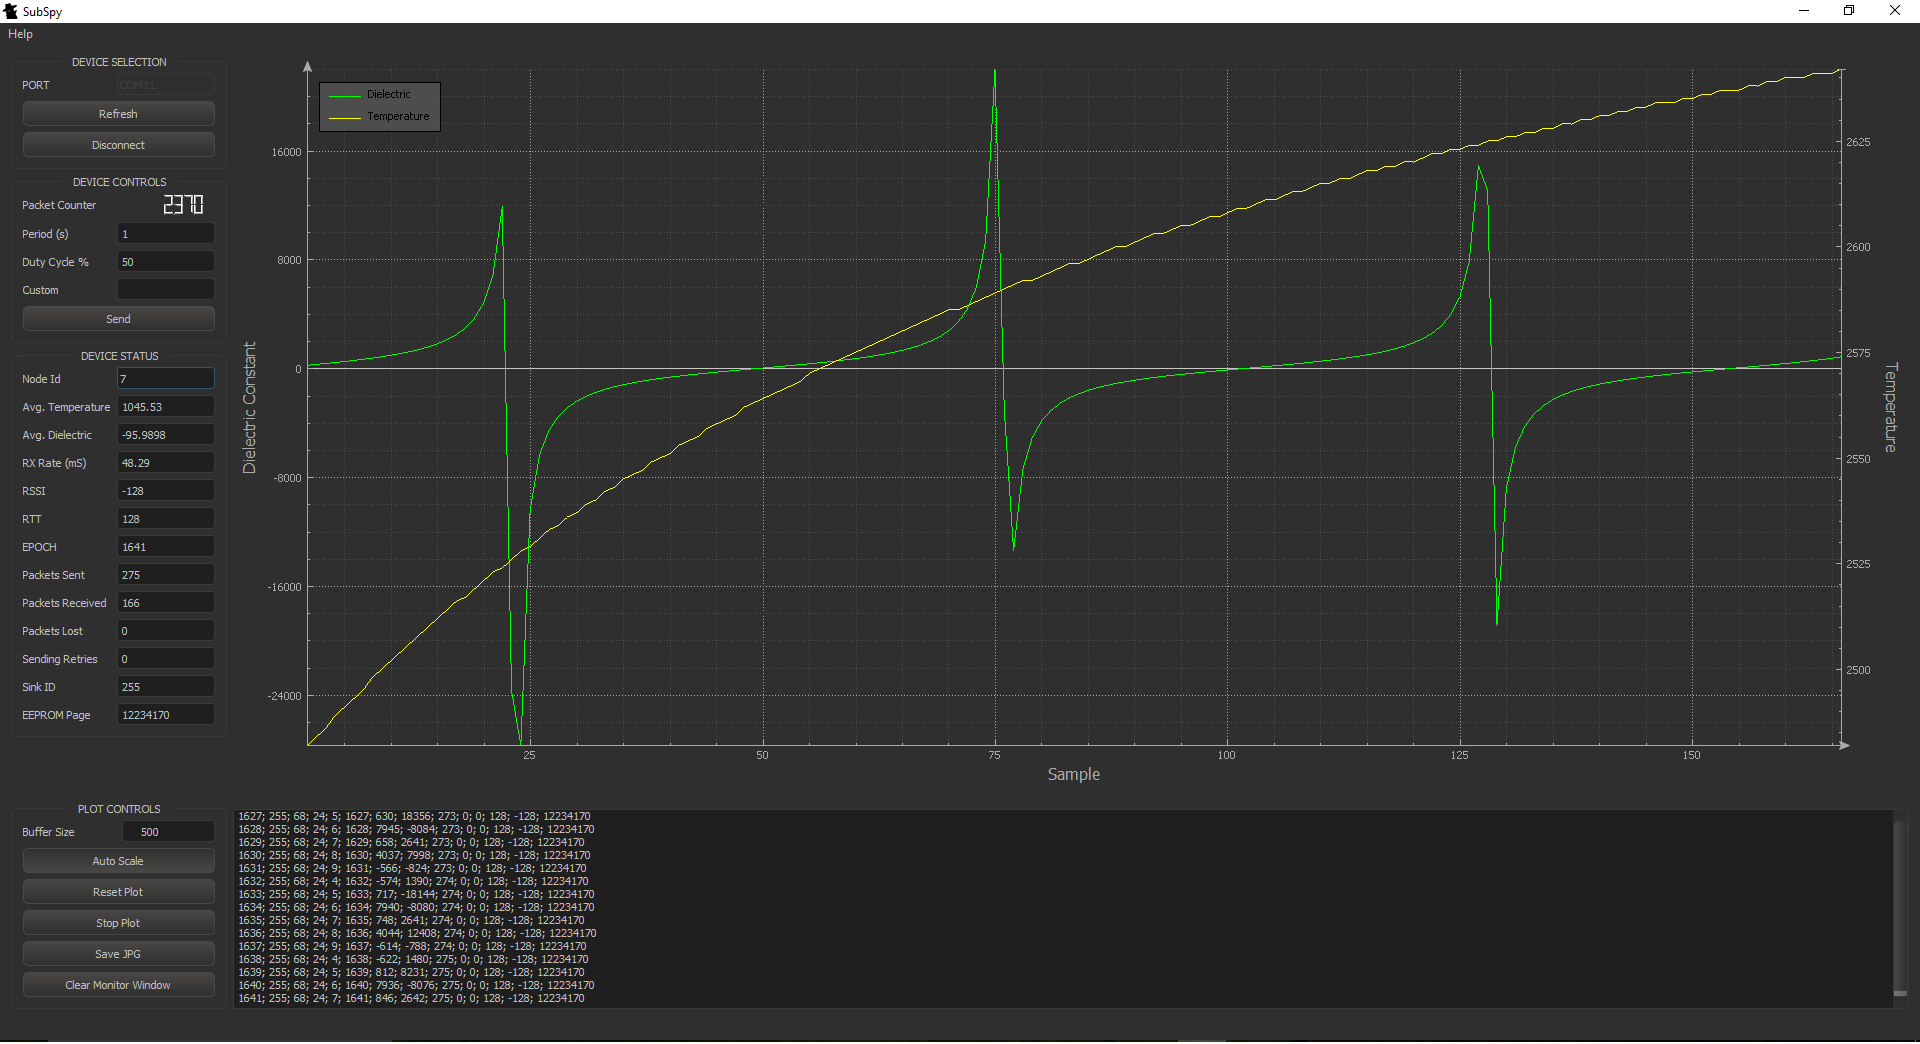
\includegraphics[width=1\textwidth]{swWindows.png}
    \caption{SubSpy windows UI screenshot.}
    \label{fig:swWindows}
\end{figure}

On the screen left top there is a combo-box which permits the user to select the wireless adapter which is mapped as a serial port (USB CDC maps as a serial port). There is one button to refresh the device listing (in case the adapter is attached after the UI has been launched) and another to connect to the spy. Below there is a packet received counter and the duty cycle configuration control together with the button to send the commands to the adapter.

In the left middle there is combo-box (Node Id) to select which device the user wants to plot the sensor readings and display the message status on the subsequent displays (all devices on the network have their data logged but the user can only plot sensor readings of one device at a time). The UI has the following message displays, which are extracted from the received data packets:
\begin{itemize}
\item Average Temperature
\item Average Dielectric
\item RX Rate (ms)
\item RSSI
\item RTT
\item Epoch
\item Packets Sent
\item Packets Received
\item Packets Lost
\item Sending Retries
\item Sink ID
\item EEPROM Page
\end{itemize}

On the left bottom are the plot controls which allow the user to activate the graph auto scaling function, reset the plot, stop plotting, save a screen shot in JPG format or clear the log window on the right. The log window displays all packets captured by the wireless adapter, not only the ones filtered by the Node Id combo-box.

Last but not least, in the center of the screen there is the plot area, QCustomPlot class has been used to implement the graph and it features a very flexible tool for data visualization. Since there are two sensor's readings being plotted, there are two vertical axes, the left one is scaled according to the dielectric constant and the right one according to the temperature. The plot can be either automatically scaled or adjusted by the user through zoom in all axes, all accomplished by mouse interaction.

Since the hardware is also compatible with android devices, a demo application has also been developed in JAVA to demonstrate compatibility, however, time constraints have prevented the application to be finalized for the IoT competition and therefore it is not on the scope of this report.

\newpage
\section{Power Consumption Evaluation}
\label{powerConsumptionEvaluation}
After completing the solution, energy consumption has been evaluated in order to guarantee that all expectations related to current draw were consolidated on the prototype. To accomplish the current measurements the tool known as EnergyTrace from Texas Instruments has been used. All the measurements referred on this report have an accuracy of $\pm 500nA \pm 2\%$. Keep in mind that all measurements must also add 7mA current offset which is the current draw from the 5V VUSB bus which supplies the USB physical layer. Figure~\ref{fig:completeCurrentProfile} depicts the current draw in different operation modes, logged with EnergyTrace device.

\begin{figure}[H]
    \centering
    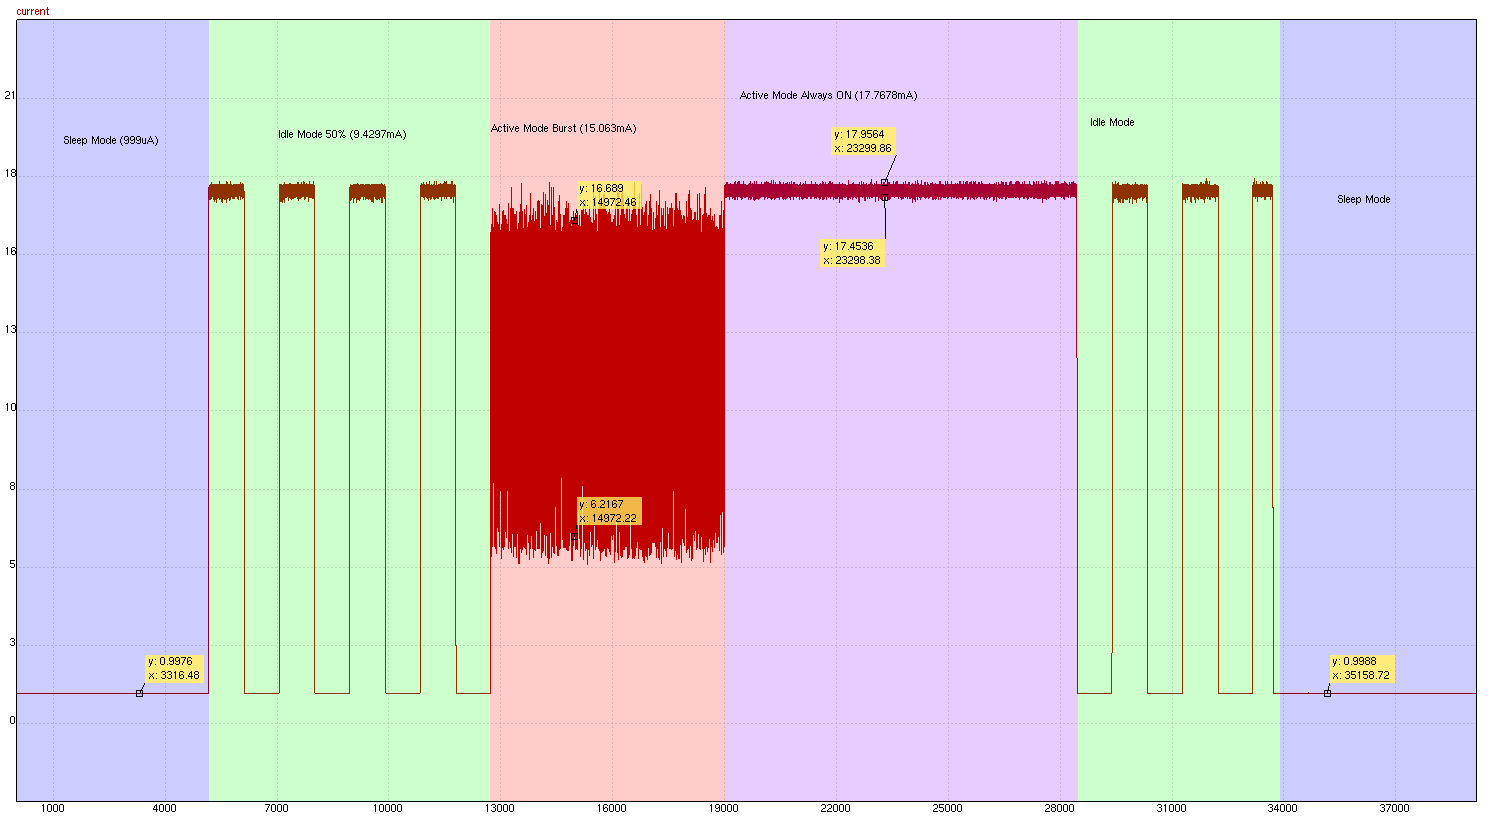
\includegraphics[width=1\textwidth]{completeCurrentProfile.png}
    \caption{Current profile.}
    \label{fig:completeCurrentProfile}
\end{figure}

On the use case illustrated on figure~\ref{fig:completeCurrentProfile}, the system is configured with a radio duty cycle of 50\%, the wireless adapter starts in sleeping mode until the the user connects to it through the GUI, from this point on the spy starts listening for packets with the configured duty cycle. This process goes on until network activity is detected, in this case the program switches to active listening mode meaning that the radio is always on. If network activity ceases, the radio keeps actively listening (100\% duty cycle) for 10 seconds until it switches back to the user configured duty cycle. Shortly after that the user disconnects the application from the wireless adapter and the spy resumes sleep mode.
As can be observed on figure~\ref{fig:completeCurrentProfile}, during packet reception (between samples 13000 and 19000, red area on the graph) the current consumption oscillates between ~17mA and ~5mA. This current oscillation is due to the implemented technique to put the radio in sleep mode while reading the received packet. 

\newpage
Figure~\ref{fig:zoomBurst} shows a zoom in the active mode burst to illustrate the radio going to sleep while its SPI interface is busy. Unfortunately the available version of EnergyTrace only has a sample frequency of 1KHz and therefore the real current draw shape cannot be precisely observed since its dynamics are faster than the sample frequency of the measuring device.

\begin{figure}[H]
    \centering
    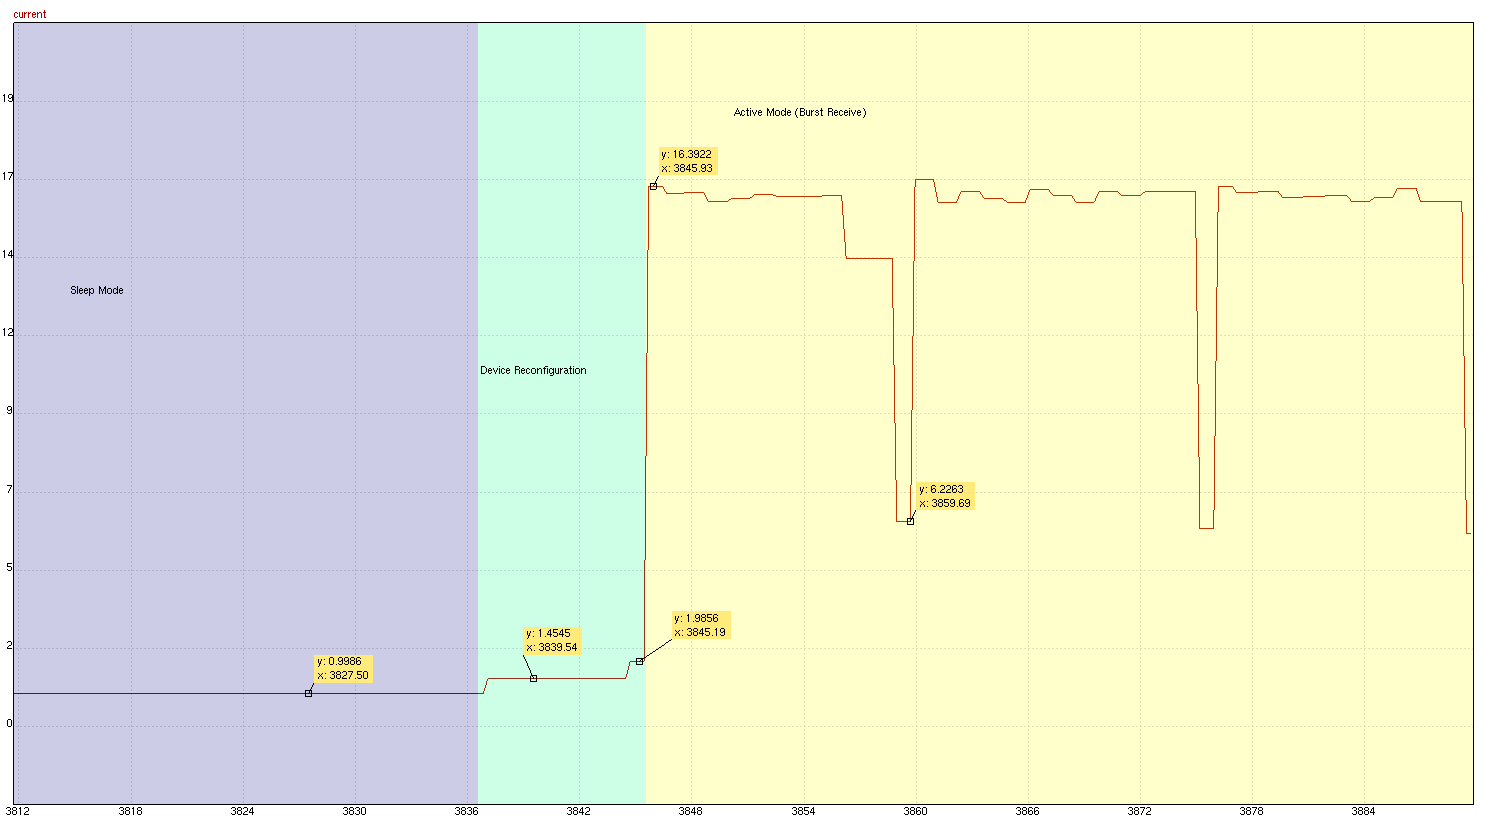
\includegraphics[width=1\textwidth]{zoomBurst.png}
    \caption{Zoom on current profile in RX mode.}
    \label{fig:zoomBurst}
\end{figure}

Finally it is possible to state that the current consumption has met all the expectations from the manufacturer's datasheet and therefore the implementation is complete and attending the power consumption constraints.

\newpage
\section{Conclusion}
\label{conclusion}
In conclusion, this report presents relevant evidence that the proposed design can attend all project requirements excelling in system performance(packet throughput), GUI friendliness (as voted on the challenge), energy consumption and implementation cost. The next step is to build the first version of the designed hardware and extend the functionalities which could not be developed on the prototype.

\newpage

\section{References}
\label{references}
\begin{thebibliography}{9}

\bibitem{msp430f5529datasheet}
  \textit{MPS430F5529 Datasheet},
  Texas Instruments,
  March 2009 – Revised November 2015.
  
\bibitem{RFM69CWdatasheet}
  \textit{RFM69CW Datasheet},
  HOPERF Microelectronics CO.

\bibitem{userGuideF5}
  \textit{MSP430X5XX and MSP430X6XX Family User's Guide},
  Texas Instruments,
  June 2008 – Revised October 2016.

\bibitem{appReport}
  Somshubhra Paul and Dung Dang,
  \textit{Maximizing MSP432P4xx Voltage Regulator Efficiency: DC-DC and LDO Features and Tradeoffs},
  Application Report,
  Texas Instruments,
  March 2015.

\bibitem{macProt}
  Hans-Christian Halfbrodt,
  \textit{Mac Protocols for Wireless Sensor Networks},
  Freie Universit{\"a}t Berlin, Germany,
  January 2010.


\end{thebibliography}

\end{document}
